\documentclass{article}

% Language setting
% Replace `english' with e.g. `spanish' to change the document language
\usepackage[english]{babel}

% Set page size and margins
\usepackage[a4paper,top=2cm,bottom=2cm,left=3cm,right=3cm,marginparwidth=1.75cm]{geometry}

% Useful packages
\usepackage{amsmath}
\usepackage{amsfonts} 
\usepackage{graphicx}
\usepackage[colorlinks=true, allcolors=blue]{hyperref}
\usepackage{listings}
\usepackage[usenames,dvipsnames]{color}    
\definecolor{backcolour}{rgb}{0.95,0.95,0.92}
\lstset{ 
  language=R,                     % the language of the code
  basicstyle=\ttfamily\scriptsize, % the size of the fonts that are used for the code
  numbers=left,                   % where to put the line-numbers
  numberstyle=\tiny\color{Blue},  % the style that is used for the line-numbers
  stepnumber=1,                   % the step between two line-numbers. If it is 1, each line
                                  % will be numbered
  numbersep=5pt,                  % how far the line-numbers are from the code
  backgroundcolor=\color{backcolour},  % choose the background color. You must add \usepackage{color}
  showspaces=false,               % show spaces adding particular underscores
  showstringspaces=false,         % underline spaces within strings
  showtabs=false,                 % show tabs within strings adding particular underscores
  frame=false,                   % adds a frame around the code
  rulecolor=\color{black},        % if not set, the frame-color may be changed on line-breaks within not-black text (e.g. commens (green here))
  tabsize=2,                      % sets default tabsize to 2 spaces
  captionpos=b,                   % sets the caption-position to bottom
  breaklines=true,                % sets automatic line breaking
  breakatwhitespace=false,        % sets if automatic breaks should only happen at whitespace
  keywordstyle=\color{RoyalBlue},      % keyword style
  commentstyle=\color{YellowGreen},   % comment style
  stringstyle=\color{ForestGreen}      % string literal style
} 


%-------------------------------------------------------------

\title{ST425 Exercise XX}
\author{You}
\date{}
\begin{document}
\maketitle


%-------------------------------------------------------------
\section*{Question 1}

\subsection*{1(a)}
The mean of a random variable $X$, of which support is $(-\infty,\infty)$, can be obtained by
\begin{equation*}
    \mathbb{E}(X) = \int_{-\infty}^{\infty}f(x)dx       
\end{equation*}
where $f(x)$ is the pdf.

\subsection*{1(b)}
Adding aligned equations. 
\begin{align*}
    \text{Var}(x) &= \mathbb{E}\left[(X-\mathbb{E}(X))(X-\mathbb{E}(X))\right] \\
                  &= \mathbb{E}(X^2) - \left(\mathbb{E}(X)\right)^2
\end{align*}


%-------------------------------------------------------------
\newpage
\section*{Question 2}

\subsection*{2(a)} 
Adding R code.
\begin{lstlisting}
    library(ggplot2)
    set.seed(1234)
    
    n <- 1000
    x_norm1 <- rnorm(n = n, mean = 0, sd = 1)
    x_norm2 <- rnorm(n = n, mean =1, sd = 2)
    dat <- data.frame(dist = factor(rep(c("mu=0 sig=1","mu=1 sig=2"), each = n)),
                      x = c(x_norm1, x_norm2))
    
    p<-ggplot(dat, aes(x=x, fill = dist, color = dist)) +
      geom_histogram(aes(y=..density..), binwidth=.4, alpha=.5, position="identity") +
      geom_density(alpha=.3)
    p 
\end{lstlisting}

\subsection*{2(b)}
Adding figures.
\begin{figure}[h]
\centering
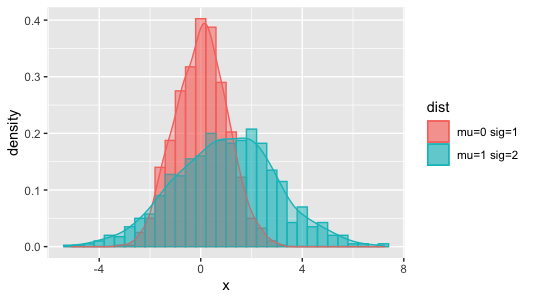
\includegraphics[width=0.6\textwidth]{Rplot.png}
\caption{R plot}
\label{fig:result}
\end{figure}
%-------------------------------------------------------------

\end{document}